\documentclass[tikz]{standalone}
\usepackage{pgfplots}
\usepgfplotslibrary{groupplots}
\pgfplotsset{width=7.cm, height=7cm, compat=1.18}
\usepackage{tikz}
\usepackage{amsmath}
\usepackage{amssymb}

\definecolor{darkgray176}{RGB}{176,176,176}

\begin{document}
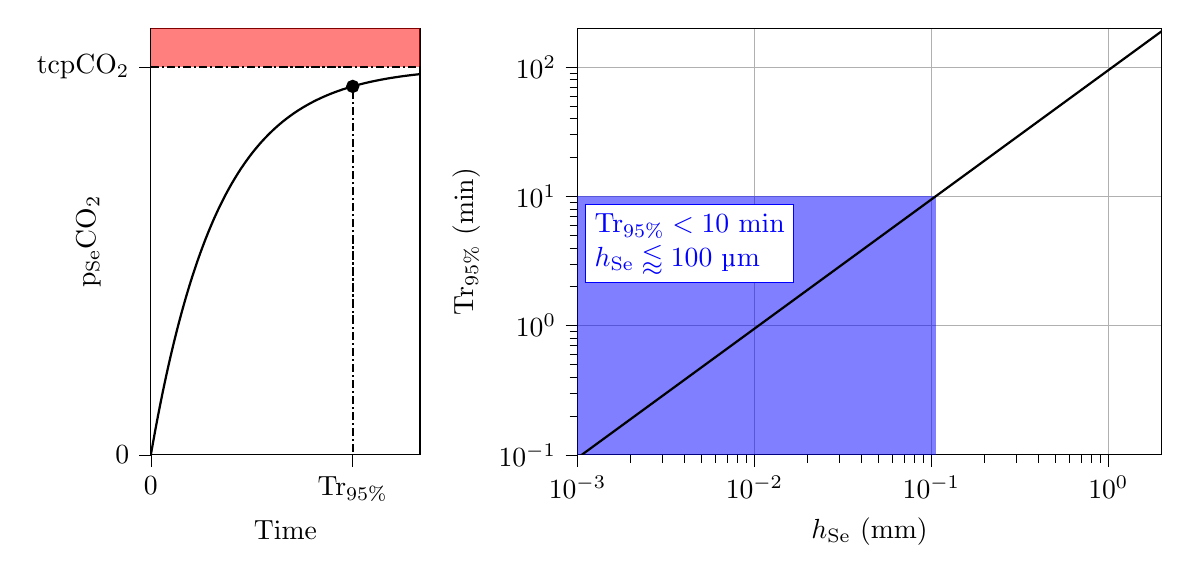
\begin{tikzpicture}
\definecolor{darkgray176}{RGB}{176,176,176}
\begin{groupplot}[group style={group size=2 by 1, horizontal sep=2cm}]
\nextgroupplot[
tick align=outside,
tick pos=left,
x grid style={darkgray176},
y label style={at={(axis description cs:-0.15,0.5)},anchor=south},
xlabel={Time},
xmin=0, xmax=4,
xtick style={color=black},
xtick={0,3},
xticklabels={0,Tr$_{95\%}$},
ytick={0,1},
yticklabels={0,tcpCO$_2$},
y grid style={darkgray176},
ylabel={p$_\text{Se}$CO$_2$},
ymin=0., ymax=1.1,
ytick style={color=black},
width=5cm,
]
\draw[draw=none, fill=red, fill opacity=0.5] (0,1) rectangle ++(4,-0.05);
\addplot[domain = 0:4,	samples = 200, smooth,
thick] {1-exp(-x)};
\addplot [thick, densely dashdotted, mark=*, mark options={fill=black, draw=none, solid}] table {%
	3 -0.2
	3 0.95
	};
\addplot[domain = 0:4,	samples = 2, thick, densely dashdotted] {1};

% ---------------------
\nextgroupplot[
tick align=outside,
tick pos=left,
x grid style={darkgray176},
y label style={at={(axis description cs:-0.15,0.5)},anchor=south},
xlabel={$h_\text{Se}$ (mm)},
xmin=1e-3, xmax=2,
xtick style={color=black},
y grid style={darkgray176},
ylabel={Tr$_{95\%}$ (min)},
ymin=0.1, ymax=2E2,
ytick style={color=black},
ymode=log,
xmode=log,
width=9cm,
grid=major,
]
\draw[draw=none, fill=blue, fill opacity=0.5] (1e-3,1e-1) rectangle ++(100/0.94737,100);
\addplot[domain = 0.5e-3:4,	samples = 2, thick] {94.737*x};
\node[anchor=north west, blue, align=left, fill=white, draw=blue] at (0.0011, 8.7)
{Tr$_{95\%} < 10$~min\\ $h_\text{Se} \lessapprox 100$~{\textmu}m};
\end{groupplot}
\end{tikzpicture}
\end{document}